\documentclass{article}

\usepackage[utf8]{inputenc}
\usepackage[margin=1in]{geometry}
\usepackage[colorlinks=true, pdfborder={0 0 0}]{hyperref} 
\usepackage{microtype}
\usepackage{amsfonts}
\usepackage{amssymb}
\usepackage{graphicx}
\usepackage{subfig}
\usepackage{float}
\usepackage{siunitx}
\usepackage{listings}
\setcounter{topnumber}{8}
\setcounter{bottomnumber}{8}
\setcounter{totalnumber}{8}
\usepackage{arydshln}
\usepackage[framemethod=tikz]{mdframed}
\usepackage{minted}
\usepackage{empheq}
\usepackage{nicematrix}
\usepackage{titlesec}

\usepackage[sorting=nty]{biblatex}
\addbibresource{sources.bib}

\setlength{\parindent}{0cm}
\setlength{\leftskip}{0cm}

\usepackage{amsmath}
% For annet format på formler:
% \usepackage[fleqn]{amsmath}
% \setlength{\mathindent}{0cm}

\lstset{
  language=Python,
  basicstyle=\footnotesize\ttfamily,
  %keywordstyle=\color{blue},
  %commentstyle=\color{green},
  %stringstyle=\color{red},
  numbers=left,
  numberstyle=\tiny,
  numbersep=5pt,
  breaklines=true,
  showstringspaces=false,
  xleftmargin=.25in,
  xrightmargin=.25in
}

\definecolor{barcolor}{rgb}{0,0,0}
\renewenvironment{leftbar}[1][\hsize]{
    \def\FrameCommand{{\color{barcolor}\vrule width 0.5pt \hspace{10pt}}}
    \MakeFramed{\hsize#1 \advance\hsize-\width \FrameRestore}
}{\endMakeFramed}

\titleformat{name=\section,numberless}[block]
  {\normalfont\Large\bfseries}
  {\llap{\rule[0ex]{0.6em}{0.6em}\hspace{1.8em}}}{0em}{\titlerule\\[.8ex]}{}

\renewcommand\thefootnote{\textcolor{black}{\arabic{footnote}}}
\renewcommand{\footnoterule}{}

\setlength{\parskip}{0.15cm}

\begin{document}

\begin{center}
    \textbf{\LARGE REINFORCEMENT LEARNING}

    %\rule{4cm}{1pt}
    \vspace{0.2cm}

    2024

\end{center}

\section*{MOTIVATION}

Reinforcement learning is a powerful approach in machine learning where an artificial neural network (hereafter "Agent") learns to make decisions by interacting with an environment. The Agent receives feedback, either instantaneously or with a delay, based on its actions. This feedback, also known as the "reward", guides the Agent in learning the optimal actions to take in different situations or "states" within the environment.

Initially, an Agent starts with no knowledge of the environment and must learn through trial and error which actions lead to positive rewards. This learning process involves adjusting the weights of the Agent over many iterations to improve its performance on the task at hand. This process may in some cases be challenging, especially if the reward is significantly delayed - which makes it hard for the Agent to determine which of its actions led to the reward.

An example of extremely delayed feedback is OpenAIs work on mastering Minecraft. They had a goal for their Agent to obtain diamond tools, which "usually takes proficient humans over 20 minutes (24,000 actions)". They achieved this through sequentially rewarding the Agent based on the progress it made, thus providing it with more immediate feedback based on its actions. \cite{Minecraft}

\section*{REINFORCEMENT LEARNING APPROACHES}

For any given reinforcement Agent, the goal is to select the action that will yield the highest reward. In order to best learn how to predict the correct actions, various approaches can be taken.

\subsection*{Policy-based}
\begin{leftbar}
    The policy, $\pi(a|s)$, of an Agent is the probabilities of selecting the different possible actions $a$ given a state $s$. Therefore, finding the optimal policy $\pi^*(a|s)$ which maximizes the expected rewards given the current state is what the Agent leans to do. \cite{HF-approaches}

    Performance of the Agent is optimized based on the probability distribution of the possible actions given a state with respect to its parameters. This optimization is based on the Agent's experience, in order to obtain a gradient which can then directly influence the parameters. \cite{HF-policy}

    \hypertarget{sec:policy-based-approach}{}
    \subsubsection*{PROCEDURE \hfill POLICY-BASED GRADIENT APPROACH}

    Weights of the Agent is updated through a modified version of the REINFORCE algorithm \cite{REINFORCE}.

    The expected future reward $R_i$ for each time step $i \in [0, N]$ is calculated as:

    \begin{equation*}
        \begin{split}
            R_i &= r_i + \gamma \times R_{i+1} \\
            R'_i &= (R_i - \mu_R) / \sigma_R
        \end{split}
    \end{equation*}

    where $r_i$ is the reward at time step $i$, and $\gamma$ is the discount factor. The expected future rewards are calculated backwards, as $R_{N+1} = 0 \Rightarrow R_N = r_N$. The expected rewards are then standardized.

    The policy gradient $G_i$ at each time step $i$ is calculated as

    \begin{equation*}
        G_i = - \log(\pi(a_i|s_i)) \times R'_i
    \end{equation*}

    where $\pi(a_i|s_i)$ is the probability of taking action $a_i$ given state $s_i$, and $R'_i$ is the standardized expected future reward. The overall gradient is the sum of these individual gradients, $G = \sum_{i}^N G_i$.

    The weights of the Agent are updated using the calculated gradient $G$ and the learning rate $\eta$:

    \begin{equation*}
        w_{new} = w_{old} - \eta \times \nabla_w G
    \end{equation*}

    where $\nabla_w G$ is the gradient of $G$ with respect to the weights $w$.

\end{leftbar}
\subsection*{Value-based}
\begin{leftbar}
    In contrast to a policy-based approach which outputs a probability distribution across the possible actions, the value-based approach outputs a predicted value of being at the given state. \cite{HF-value}

    \textbf{\textcolor{red}{NOT DONE, ADD MORE HERE}}
\end{leftbar}

\section*{AGENT ARCHITECTURE}

Where Barto, Sutton and Anderson used "two types of neuronlike adaptive elements [...] an \textit{associative search element} (ASE) and the other an \textit{adaptive critic element} (ACE)" \cite{Neuronlike}, one can achieve near-perfect behavior with simpler architectures. A simple Agent skeleton is created using \textit{torch} as seen below. Here an arbitrary number of neurons per layer is used.

\begin{lstlisting}
import torch

class Agent(torch.nn.Module):
    def __init__(self, inputs=4, outputs=2):
        super(Agent, self).__init__()

        self.layer_in = torch.nn.Linear(inputs, 20)
        self.layer_hidden = torch.nn.Linear(20, 80)
        self.layer_out = torch.nn.Linear(80, outputs)

    def forward(self, state):
        _output = torch.relu(self.layer_in(state))
        _output = torch.relu(self.layer_hidden(_output))
        output = self.layer_out(_output)

        return output

    def learn(self):
        pass
\end{lstlisting}

Note that this is an extremely simplified architecture, and that multiple hidden layers of variable units may be added, different activation functions used, etc. The above architecture being quite small is therefore not intended to generalize across tasks, but instead act as a tailored Agent for the task in question.

Also, when training the Agent, one has to determine how to calculate the gradient/loss. This can either be a generalized or tailored approach, depending on the use-case of the Agent. In the letter by Mnih \textit{et.al.} they chose an approach that generalized well across tasks; "a single algorithm that would be able to develop a wide range of competencies on a varied range of challenging tasks", as well as using a different Agent architecture \cite{Human-level}.

\subsection*{Implementation of policy-based gradient approach}
\begin{leftbar}

    For a policy-based gradient approach, \textit{i.e.} an Agent that chooses an action based on the expected reward, some additions to the Agent class above is needed.

    \subsubsection*{BEHAVIOUR MEMORY}

    The Agent's parameters are initialized as random values by default. These parameters are then updated once for every game the Agent plays (\textit{i.e.}, one full interaction with the environment). Therefore, it is necessary to store the behaviour and corresponding rewards of the Agent. Instead of saving the predicted actions, the logarithm of the probability of the chosen action is saved. The reason for this is that the logarithm of the Agent's confidence is needed for calculating the policy gradient.

    Obtaining the action and the logarithm of its probability is achieved by adding a wrapper to the forward pass given a state:

    \begin{lstlisting}
    def action(self, state):
        actions = torch.softmax(self(state), dim=-1)

        action = np.random.choice([0, 1], 1, p=actions.detach().numpy())[0]
        logarithm = torch.log(actions[action])

        return action, logarithm
    \end{lstlisting}

    Thus, the 'action' method returns the selected action and the logarithm of its probability, which are used in the learning process to update the Agent's parameters. In addition, the wrapper introduces some sense of exploration, by randomly sampling an action based on the Agent's policy.

    \subsubsection*{LEARNING}

    After every game the Agent plays (during the training-loop), its parameters are updated with respect to the policy gradient. In order for the Agent to best learn the optimal actions, it is common to evaluate the expected future rewards. Then, the Agent can adjust its predicted action probabilities (policy) so that this expected reward is maximized. See the \hyperlink{sec:policy-based-approach}{procedure} for mathematical equivalent formulas.

    The expected reward given an action is the sum of all future (discounted) rewards. This is achieved by reversely adding the observed reward and the discounted cumulative future rewards. The rewards are then standardized.

    \begin{lstlisting}
    _reward = 0
    for i in reversed(range(len(rewards))):
        _reward = _reward * self.discount + rewards[i]
        rewards[i] = _reward
    rewards = (rewards - rewards.mean()) / (rewards.std() + 1e-9)
    \end{lstlisting}

    The policy gradient is the gradient of the expected reward with respect to the action taken (policy). This is computed by multiplying the logarithm of the selected action probability (see `action` method) with the standardized expected reward — previously calculated. The overall gradient is then the sum of all these products.

    \begin{lstlisting}
    gradient = torch.zeros_like(rewards)
    for i, (logarithm, reward) in enumerate(zip(self.logarithms, rewards)):
        gradient[i] = -logarithm * reward
    gradient = gradient.sum()
    \end{lstlisting}

    A chosen optimizer is then used to backpropogate and update the Agent's parameters with the given gradient.

\end{leftbar}

The full Agent architecture can be found in the file 'reinforcement-learning/cart-pole/policy-based.ipynb'. Implementation based on Yoon's article \cite{REINFORCE}.

\subsection*{Implementation of value-based approach}
\begin{leftbar}
    \textbf{\textcolor{red}{NOT YET IMPLEMENTED}}
\end{leftbar}

\section*{CART-POLE ENVIRONMENT}

\begin{minipage}{.5\textwidth}
  To gain a basic understanding of how reinforcement learning works one can experiment with a "simple" problem. The cart-pole problem being such, is an environment where the Agent has to balance a pole on top of a cart by moving it either to the left or the right — based on the current state of the environment. In this environment, the Agent gets immediate feedback from its actions.
\end{minipage}%
\begin{minipage}{.5\textwidth}
    \centering
    
\includegraphics[width=.8\linewidth]{images/cart-pole.png}
    \captionof{figure}{Random observed environment state.}
    \label{fig:cart-pole}
\end{minipage}

\vspace{0.2cm}

The cart-pole environment (seen in Figure \ref{fig:cart-pole}) is a part of the \textit{Gymnasium} package in python. This package contains a number of different virtual environments which can be imported and used to train and validate ones own reinforcement Agents. \cite{Gymnasium} \cite{Cart-pole} The environment is created and initialized by the following lines of python code:

\vspace{0.2cm}

\begin{lstlisting}
    import gymnasium as gym
    
    environment = gym.make('CartPole-v1', render_mode="rgb_array")
    observation, info = environment.reset()
\end{lstlisting}

The Agent controls the cart movement, \textit{i.e.}, by pushing it one way or another. The action is therefore binary, being $0$ or $1$ for respectively pushing the cart to the left or the right. By being able to observe the current state of the cart position, cart velocity, pole angle and pole angular velocity, the Agent has to choose an appropriate action. A reward is given for every time-step until the pole is no longer standing. The termination (or truncation) is determined by whether the pole angle is greater than $\pm 12 ^\circ$, the cart position is more than $\pm 2.4$ (too far away), or the episode length is greater than $500$ time-steps.

\subsection*{Policy-based Agent}
\begin{leftbar}
    Training the policy-based Agent by playing $10 000$ games led to a surprisingly good performance. The Agent was trained with the \textit{RMSprop} optimizer with a learning-rate of $0.00025$ and a reward discount of $0.99$. See Figure \ref{fig:policy-based-metrics} in the \hyperlink{sec:results}{Results} section.
\end{leftbar}
\subsection*{Value-based Agent}
\begin{leftbar}
    \textbf{\textcolor{red}{NOT YET IMPLEMENTED}}
\end{leftbar}

\newpage
\hypertarget{sec:results}{}
\section*{Results}

\begin{figure}[h]
    \centering
    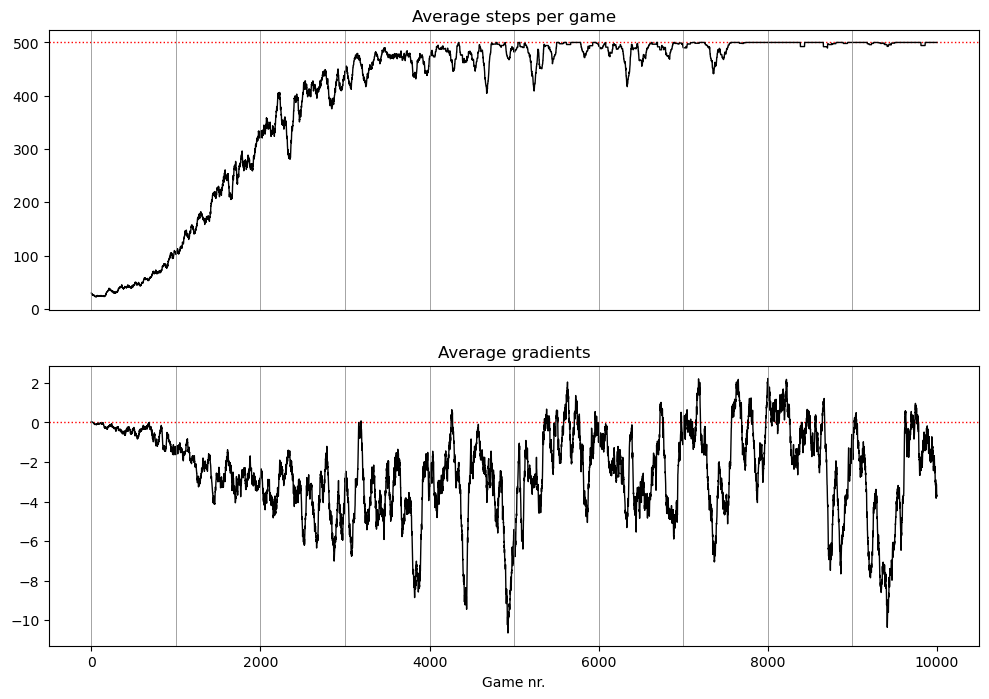
\includegraphics[width=15cm]{images/policy-based-metrics.png}
    \caption{Training of the policy-based Agent.}
    \label{fig:policy-based-metrics}
\end{figure}

\newpage
\printbibliography

\end{document}
